\begin{frame}{Portfolio Builder}
The portfolio builder builds the portfolio from the investible universe and the action from the RL model.
\\
\begin{block}{Portfolio}
The portfolio F is an m dimension vector space of weights f.
\[
    F = \{ {f \in \mathbb{R} } \} ^m,
    \sum_{i=1}^m {f_i} =1
\]
\end{block}
\begin{block}{Weight}
Weight is a real number between 0 and 1. \alert{(No short position)}
\[
    f \in \mathbb{R} | 0 \leq f \leq 1 
\]
\end{block}
\end{frame}




\begin{frame}{Trading System}
The Trading System measures performances of the given portfolios
\begin{block}{Performances}
\begin{itemize}
    \item MDD
    \item CAGR
    \item Profit
    \item Wealth
\end{itemize}
\end{block}
These performances will be the input to calculate the reward or evaluate the performance of the system. 
\end{frame}


\begin{frame}{The differential Sharpe ratio}
Online learning systems required influence on Sharpe ratio, an incremental Sharpe ratio, or differential Sharpe ratio \(D_t\).
\begin{block}{Differential Sharpe Ratio}

\[
\cfrac{d D_t}{d R_t} = 
\cfrac{B_{t-1}-A_{t-1} R_t}{(B_{t-1}-A_{t-1}^2)^\frac{3}{2}}
\]
where
A and B is the first and second moments of the returns' distributions
\[ A_n = \cfrac{1}{n}\sum_{i=1}^nR_i\quad
B_n = \cfrac{1}{n}\sum_{i=1}^nR_i^2
\]
\end{block}
\end{frame}


\begin{frame}{Differential form}
The reward function will use the differential form of the utility function \(D_t\).

\begin{block}{Differential Form}

\[
D_t = 
\begin{cases}
    \cfrac{R_{t-1} -\frac{1}{2}A_{t-1}}{DD_{t-1}},&\text{if  }R_t > 0\\
    \cfrac{DD_{t-1}^2 (R_{t-1}-\frac{1}{2}A_{t-1})  -\frac{1}{2}A_{t-1} R_t^2}{DD_{t-1}^3},&\text{if  }R_t \leq 0
\end{cases}
\]
\end{block}
Unlike utility functions that use variance as the risk-adjusted factor, this formula indicates no penalty for large positive returns. 

\end{frame}



\begin{frame}{Soft Actor-Critic}
We Use Soft Actor-Critic (SAC), as the DRL model.
\begin{block}{Actor-Critic}
     \begin{columns}
        \begin{column}{0.45\textwidth}
        \begin{enumerate}
            \item Observes the states from the environment.
            \item Performs the action on the environment.
            \item Calculate TD error based on the reward.
            \item Adjust the parameters of Value function and the policy with the TD error.
        \end{enumerate}
        \end{column}
        \begin{column}{0.45\textwidth}
        \centering
        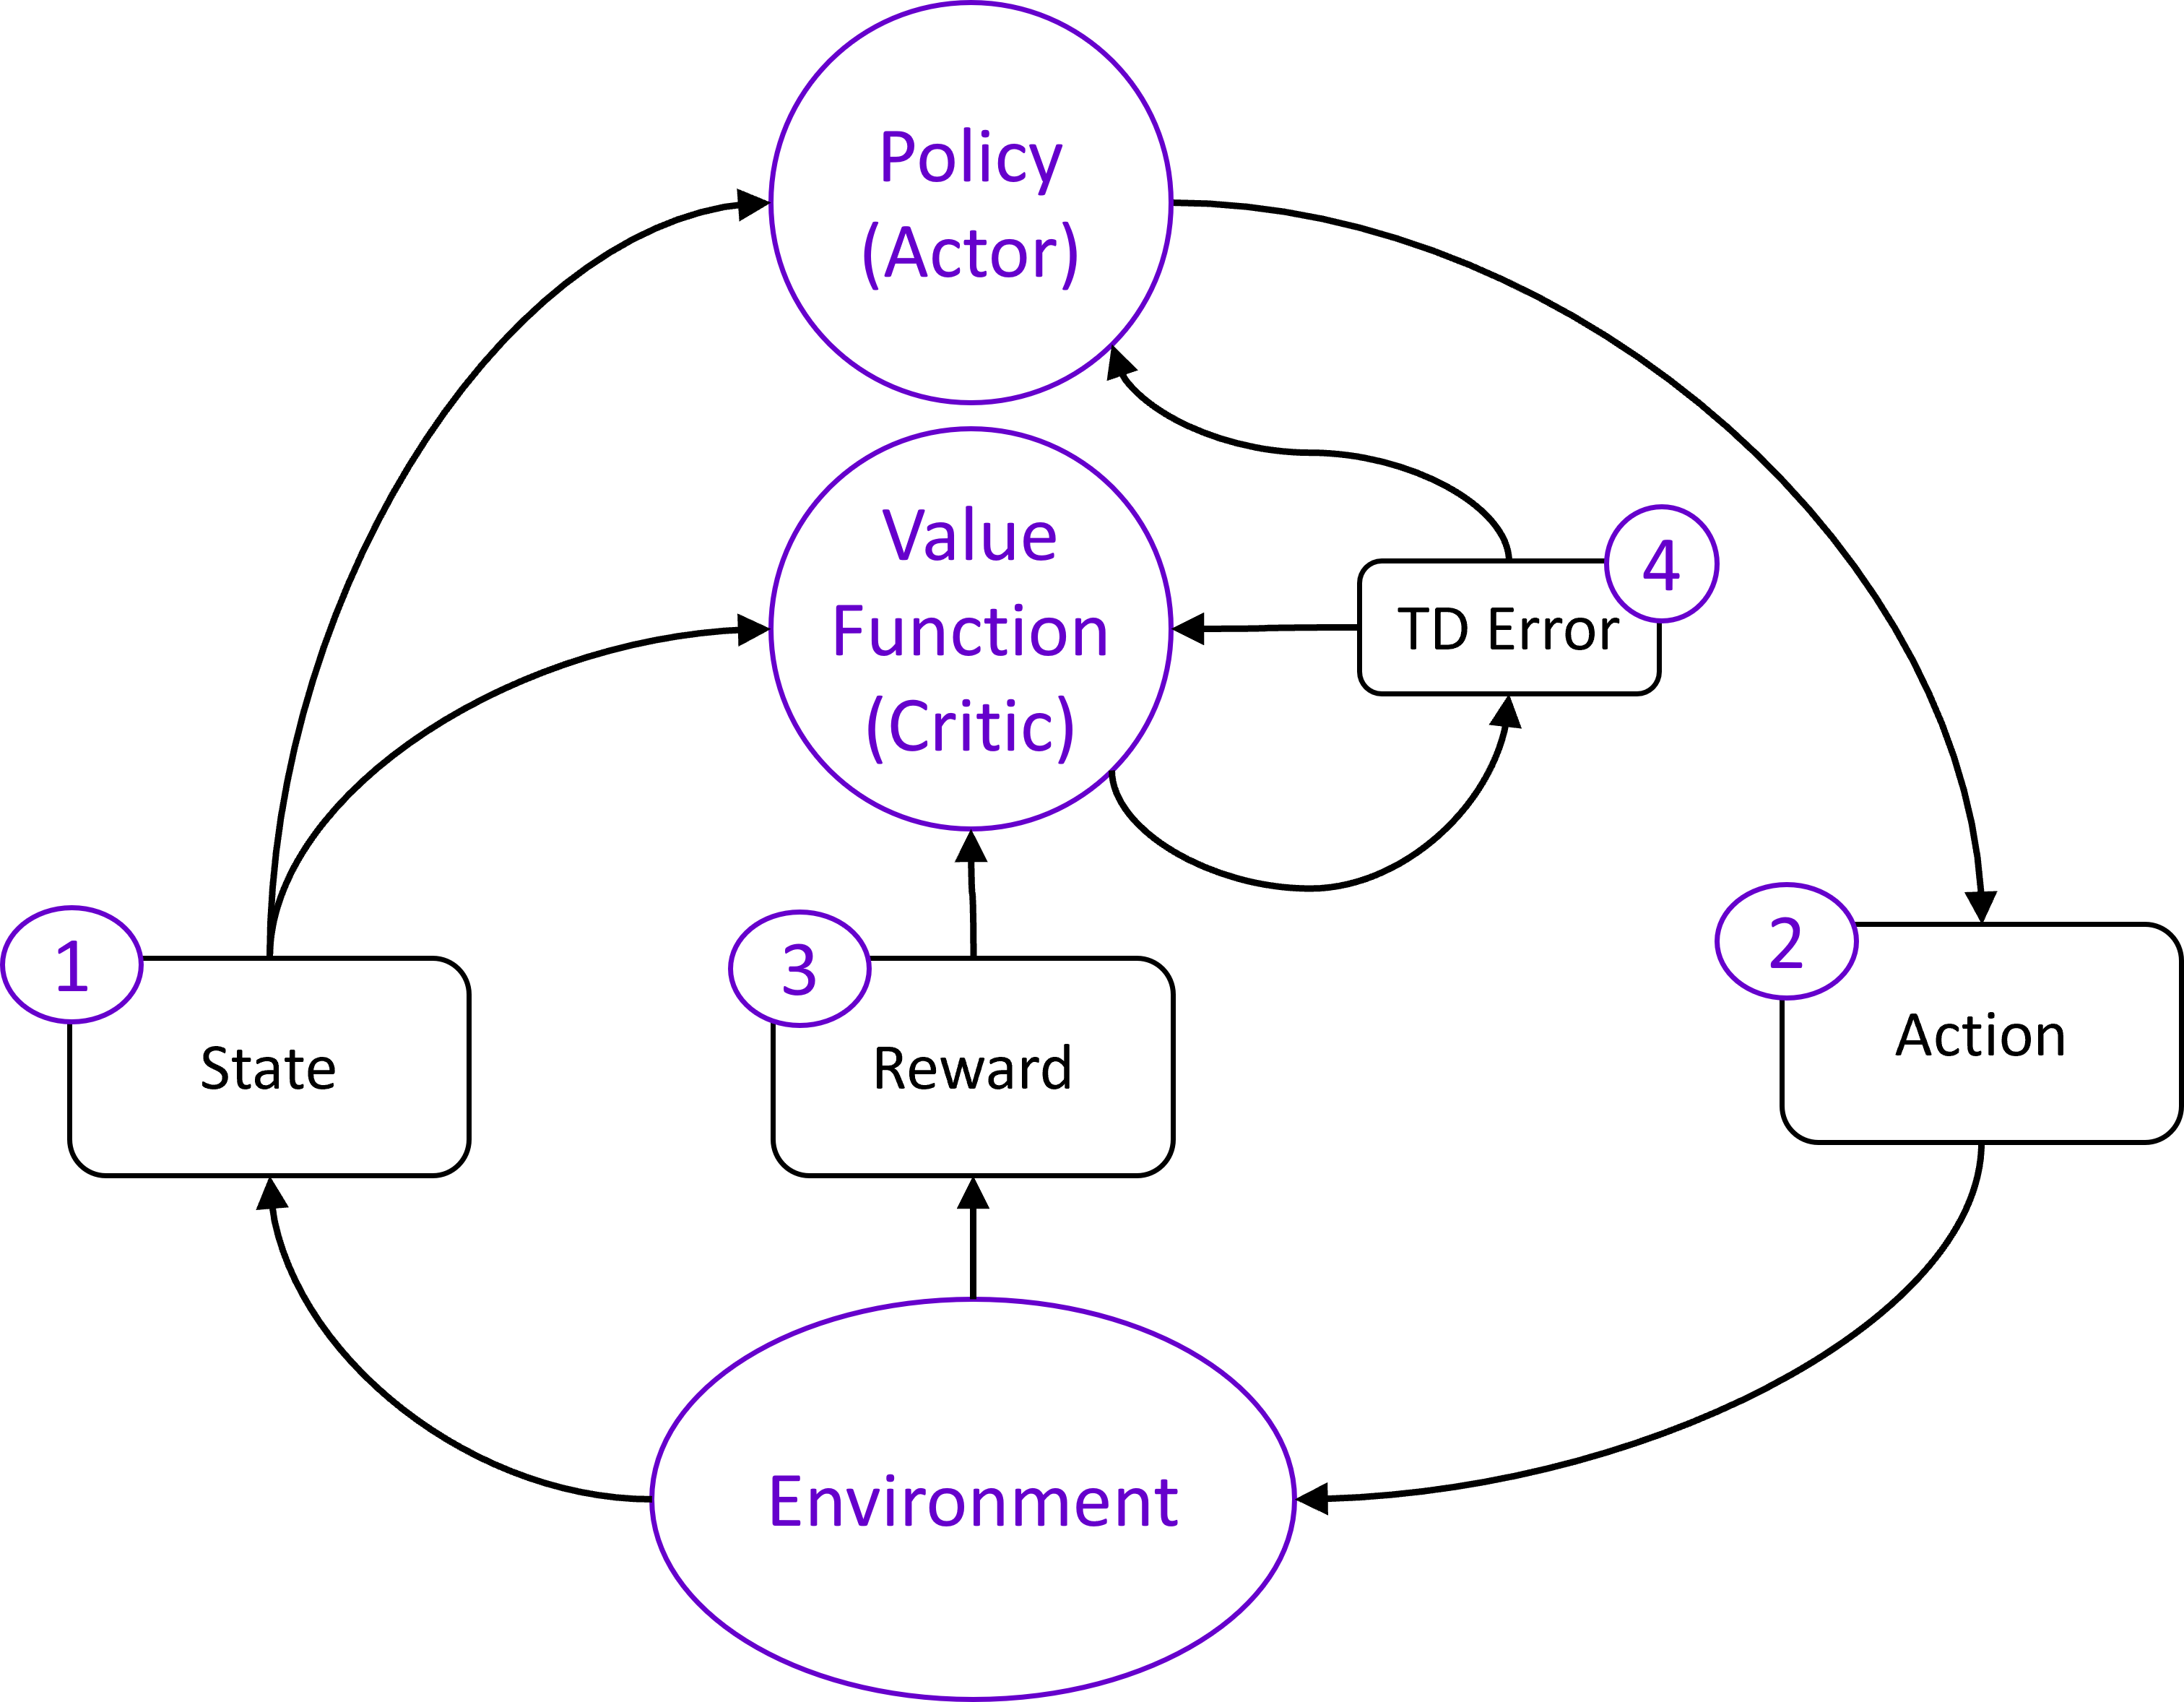
\includegraphics[width=5cm]{images/actor_critic.png}
     \end{column}
     \end{columns}
 \end{block}
\end{frame}